\documentclass[11pt]{article}
\usepackage[margin=0.72in]{geometry}
\usepackage{amsmath,amssymb,booktabs,tabularx,longtable,array}
\usepackage{graphicx,float,caption}
\usepackage[dvipsnames]{xcolor}
\usepackage{hyperref}
\usepackage{listings}
\usepackage{fancyhdr}
\usepackage{microtype}
\usepackage{enumitem}
\usepackage{tikz}
\usetikzlibrary{arrows.meta,positioning,shapes.geometric}

\definecolor{Navy}{HTML}{183B5B}
\definecolor{Teal}{HTML}{168B8B}
\definecolor{Orange}{HTML}{D98200}
\definecolor{Red}{HTML}{B33430}
\definecolor{Pale}{HTML}{EFF5F8}
\hypersetup{colorlinks=true,linkcolor=Navy,citecolor=Teal,urlcolor=Navy}
\pagestyle{fancy}
\fancyhf{}
\lhead{UNSW/Khamis QRS detector}
\rhead{audited implementation: NeuroKit2 0.2.13}
\cfoot{\thepage}
\setlength{\headheight}{14pt}
\setlist[itemize]{leftmargin=1.5em,itemsep=2pt}
\setlist[enumerate]{leftmargin=1.7em,itemsep=3pt}
\newcolumntype{Y}{>{\raggedright\arraybackslash}X}
\newcommand{\important}[1]{\begin{center}\fcolorbox{Red}{red!4}{\parbox{0.93\linewidth}{\textbf{\color{Red}#1}}}\end{center}}
\newcommand{\levelbox}[2]{\begin{center}\fcolorbox{#1}{Pale}{\parbox{0.93\linewidth}{#2}}\end{center}}
\lstset{basicstyle=\ttfamily\footnotesize,backgroundcolor=\color{Pale},frame=single,breaklines=true,columns=fullflexible,showstringspaces=false}

\title{\textbf{The UNSW/Khamis QRS Detector, Without Hand-Waving}\\
\large Child-level intuition, programmer-level implementation, professor-level audit,\\
and literal outputs from the local MIT--BIH data}
\author{RR--HRV cascade implementation report}
\date{5 August 2026}

\begin{document}
\maketitle

\important{The most important distinction: this algorithm returns a deterministic \emph{QRS-event location} \(q_i\) in a transformed feature signal.  That sample is not guaranteed to be the exact physiological R-wave apex in the raw ECG.  Moving \(q_i\) to the largest positive raw sample within \(\pm50\) ms is a separate refinement rule from Ho et al.; it is not part of the original Khamis detector and it is polarity-sensitive.}

\section*{What was actually audited}
This document is tied to the local Windows implementation, not to a generic verbal summary.  The diagnostic script reimplemented every inspected stage of NeuroKit2 0.2.13's \texttt{khamis2016} port, then required the reproduced final sample array to equal \texttt{nk.ecg\_findpeaks(..., method="khamis2016")} exactly.  Equality was obtained on MIT--BIH record 108: 1,764 events in both arrays.  The implementation is a Python port of the Khamis et al. telehealth QRS detector \cite{khamis2016telehealth,neurokitpeaksource}; Ho et al. reported the port and the later fiducial-refinement step \cite{ho2025rraccuracy}.

\begin{table}[H]
\centering
\caption{Scope and non-scope.}
\begin{tabularx}{\linewidth}{@{}p{0.28\linewidth}YY@{}}
\toprule
Question & Defensible answer & What must not be claimed \\
\midrule
Does it find QRS events? & Yes; its feature is designed to enhance rapid, large ECG deflections and it applies adaptive turning-point rules. & A detected event is not automatically a true beat in every morphology/noise state. \\
Does it return \(q_i\)? & Yes. \(q_i\) is the accepted positive turning point of the final transformed feature signal. & \(q_i\) is not invented later and is not randomized. \\
Is \(q_i\) the exact R apex? & Sometimes it is close; timing must be measured. & QRS-event detection accuracy cannot be substituted for sample-accurate fiducial accuracy \cite{porr2024jitter,reklewski2026noise}. \\
Does inversion choose polarity? & No. Running both orientations provides rival candidates. & Agreement or larger absolute amplitude does not prove which extremum is the correct clinical fiducial. \\
\bottomrule
\end{tabularx}
\end{table}

\clearpage
\section{The whole timeline in one view}
\begin{figure}[H]
\centering
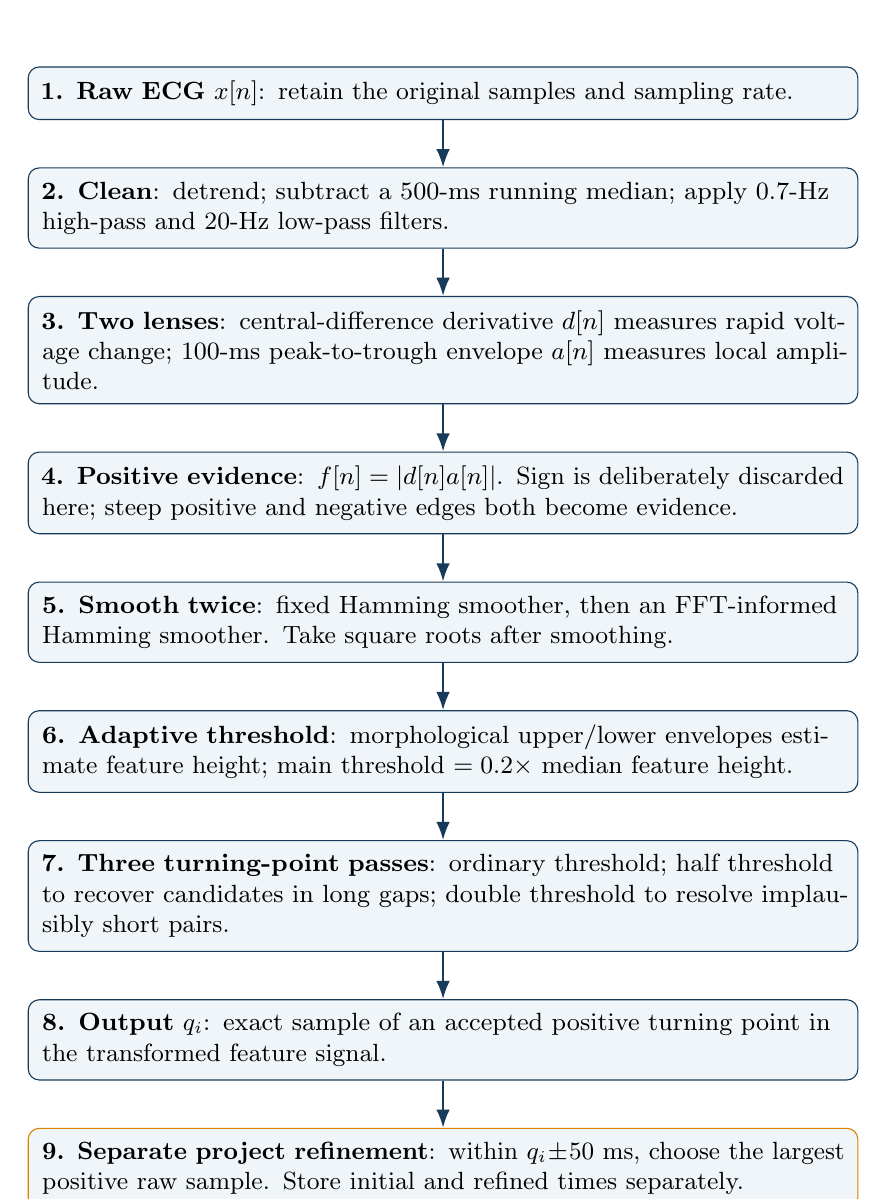
\begin{tikzpicture}[node distance=6mm,>=Latex,
box/.style={draw=Navy,rounded corners,fill=Pale,text width=0.84\linewidth,align=left,inner sep=5pt,font=\small},
arr/.style={->,thick,Navy}]
\node[box] (a) {\textbf{1. Raw ECG \(x[n]\)}: retain the original samples and sampling rate.};
\node[box,below=of a] (b) {\textbf{2. Clean}: detrend; subtract a 500-ms running median; apply 0.7-Hz high-pass and 20-Hz low-pass filters.};
\node[box,below=of b] (c) {\textbf{3. Two lenses}: central-difference derivative \(d[n]\) measures rapid voltage change; 100-ms peak-to-trough envelope \(a[n]\) measures local amplitude.};
\node[box,below=of c] (d) {\textbf{4. Positive evidence}: \(f[n]=|d[n]a[n]|\).  Sign is deliberately discarded here; steep positive and negative edges both become evidence.};
\node[box,below=of d] (e) {\textbf{5. Smooth twice}: fixed Hamming smoother, then an FFT-informed Hamming smoother.  Take square roots after smoothing.};
\node[box,below=of e] (f) {\textbf{6. Adaptive threshold}: morphological upper/lower envelopes estimate feature height; main threshold \(=0.2\times\) median feature height.};
\node[box,below=of f] (g) {\textbf{7. Three turning-point passes}: ordinary threshold; half threshold to recover candidates in long gaps; double threshold to resolve implausibly short pairs.};
\node[box,below=of g] (h) {\textbf{8. Output \(q_i\)}: exact sample of an accepted positive turning point in the transformed feature signal.};
\node[box,below=of h,draw=Orange] (i) {\textbf{9. Separate project refinement}: within \(q_i\pm50\) ms, choose the largest positive raw sample.  Store initial and refined times separately.};
\foreach \u/\v in {a/b,b/c,c/d,d/e,e/f,f/g,g/h,h/i}{\draw[arr] (\u)--(\v);}
\end{tikzpicture}
\caption{Exact processing order of the inspected implementation plus the separately identified Ho/project refinement.}
\end{figure}

\clearpage
\section{Explain it to a child}
\levelbox{Teal}{\textbf{The flashlight story.} Imagine a long, bumpy road.  A heartbeat's QRS complex is usually a steep hill or valley.  The algorithm first removes slow hills caused by the road itself.  Then it shines two flashlights: one asks ``did the road change height very quickly?'' and the other asks ``was the local hill-to-valley swing large?''  Multiplying the answers makes genuine sharp, large events bright.  Smoothing turns several bright edge flashes from one QRS into one broad hill.  The algorithm places \(q_i\) on the top of that \emph{new hill}.}

The new hill is made from the ECG, but it is not the ECG.  Its top can be a few samples before or after the raw R apex.  At 360 samples/s, one sample is (1000/360=2.78) ms.  A five-sample displacement is therefore 13.9 ms.

\begin{figure}[H]
\centering
\includegraphics[width=\linewidth]{figures/unsw_record108_j_transformations.png}
\caption{Literal transformation of the expert \(j\) beat at sample 435,657 in local MIT--BIH record 108.  The bottom panel distinguishes the transformed-feature event \(q_i\), the expert reference and the later positive refinement.}
\end{figure}

\important{Not random does not mean exact.  The same input always gives the same \(q_i\), yet \(q_i\) can be systematically displaced because filtering, multiplication and smoothing change where the transformed hill reaches its maximum.}

\clearpage
\section{Explain it to a programmer: preprocessing}
Let \(x[n]\) be the raw ECG and \(f_s\) the sampling rate.  For record 108, \(f_s=360\) Hz.

\subsection{Detrend and running-median baseline}
A linear trend is removed first.  The implementation then computes the 50th percentile in a 500-ms window:
\[
b[n]=\operatorname{median}\{x_d[k]:k\in W_{500\mathrm{ms}}(n)\},\qquad
x_m[n]=x_d[n]-b[n].
\]
At 360 Hz the window contains 180 samples.  Child interpretation: \(b[n]\) is the slowly moving floor; subtracting it keeps the fast heartbeat shape while reducing slow baseline wander.

\subsection{Frequency filtering}
The inspected port applies a seventh-order zero-phase high-pass Butterworth filter at 0.7 Hz and a seventh-order zero-phase low-pass Butterworth filter at 20 Hz.  Zero-phase forward/backward filtering avoids the ordinary causal phase delay in this offline analysis, but boundary effects and morphology-dependent changes remain.  This is consistent with the Khamis detector design for clinical and telehealth ECG \cite{khamis2016telehealth,neurokitpeaksource}.

\begin{lstlisting}[caption={Programmer-level skeleton; exact helper details are documented later.}]
detrended = scipy.signal.detrend(ecg)
baseline = running_percentile(detrended, 500_ms, percentile=50)
median_removed = detrended - baseline
highpassed = butterworth_zero_phase(median_removed, order=7, highpass=0.7_Hz)
filtered = butterworth_zero_phase(highpassed, order=7, lowpass=20_Hz)
\end{lstlisting}

\subsection{Why this is not innocuous}
Preprocessing is part of the detector definition.  Changing cutoff, order, sampling-rate handling or causal versus zero-phase filtering creates a different algorithm.  The inspected NeuroKit port also documents boundary-padding differences from the historical MATLAB percentile filter \cite{neurokitpeaksource}.  Exact reproduction therefore means exact software version and parameter logging, not merely writing ``UNSW detector.''

\clearpage
\section{Explain it to a programmer: the feature signal}
\subsection{The derivative is a central finite difference}
The coefficient vector is
\[
h_d=\frac{[1,0,-1]}{2(1/f_s)}=\frac{f_s}{2}[1,0,-1].
\]
Ignoring the causal filter's indexing convention, this approximates the local rate of change:
\[
d[n]\approx\frac{x_f[n+1]-x_f[n-1]}{2/f_s}.
\]
A positive value means voltage is rising; a negative value means it is falling; magnitude means steepness.

\subsection{The 100-ms amplitude envelope}
Within 100 ms (36 samples at 360 Hz), compute
\[
a[n]=\max_{k\in W(n)}x_f[k]-\min_{k\in W(n)}x_f[k].
\]
This is local peak-to-trough range, not a probabilistic confidence and not the later HR slope feature.  Derivative and envelope are two mathematical views of the same ECG: rate of change versus local voltage span.

\subsection{Multiply and discard sign}
\[
f[n]=|d[n]a[n]|.
\]
Because \(a[n]\ge0\), the absolute value makes both a steep rise and a steep fall positive evidence.  This gives the \emph{event detector} partial polarity robustness.  It does not make the final raw-ECG fiducial selection polarity-aware.

\begin{table}[H]
\centering
\caption{A literal toy calculation at 360 Hz.}
\begin{tabular}{@{}rrrrr@{}}
\toprule
\(x_f[n-1]\) & \(x_f[n+1]\) & \(d[n]\) & \(a[n]\) & \(f[n]=|da|\) \\
\midrule
0.10 mV & 0.50 mV & \(72.0\) mV/s & 0.80 mV & 57.6 \\
0.50 mV & 0.10 mV & \(-72.0\) mV/s & 0.80 mV & 57.6 \\
0.20 mV & 0.22 mV & \(3.6\) mV/s & 0.10 mV & 0.36 \\
\bottomrule
\end{tabular}
\end{table}
The first two rows have opposite directions but identical evidence after the absolute value.  The last row changes slowly and remains weak.

\clearpage
\section{Explain it to a programmer: smoothing and rate adaptation}
The first Hamming FIR smoothing design uses a nominal cutoff of 6 Hz.  On record 108 this produced 40 coefficients.  The filtered feature is made positive and square-root compressed:
\[
s_1[n]=\sqrt{|\operatorname{filtfilt}(h_{40},f)[n]|}.
\]

The code splits the signal into 2-s sections, removes each section's mean, calculates a 16,384-point FFT, normalizes each spectrum by its total magnitude, and averages.  It searches 0.1--4 Hz for the largest spectral component.  This is an internal estimate of repeated QRS-event frequency, not the final patient heart rate.

For record 108 the selected component was 0.98877 Hz, numerically \(60\times0.98877=59.33\) cycles/min.  The second smoother uses
\[
f_c=\operatorname{median}\bigl(2[1.5,f_{\mathrm{FFT}},4.0]\bigr).
\]
Because multiplying all three numbers by two also doubles their median, \(f_c=2\times\operatorname{median}(1.5,0.98877,4)=3.0\) Hz.  This generated an 80-coefficient Hamming smoother in this record.

\begin{figure}[H]
\centering
\includegraphics[width=0.94\linewidth]{figures/unsw_frequency_adaptation.png}
\caption{Literal record-108 spectrum used by the detector.  The selected 0.9888-Hz component is below the 1.5-Hz lower design value, so the median rule yields a 3-Hz second smoothing setting.}
\end{figure}

\important{The FFT does not create RR intervals and does not label tachycardia.  It only adapts a smoother used before event thresholding.  Actual BPM is later calculated from consecutive selected fiducials as \(60f_s/(r_i-r_{i-1})\).}

\clearpage
\section{Explain it to a programmer: adaptive turning points}
The final feature \(s_2[n]\) receives a morphological upper and lower envelope.  In record 108 the window was 720 samples, or 2.0 s.  Define
\[
H=\operatorname{median}(U[n]-L[n]),\qquad \theta=0.2H.
\]
Literal values were \(H=3.18554\) and \(\theta=0.63711\) in feature units.

\subsection{What is a turning point?}
A local peak changes direction from rising to falling; a trough changes from falling to rising.  The helper walks between alternating peaks and troughs and ignores tiny reversals whose height difference does not exceed the threshold.  Positive returned indices are feature peaks; negative values encode troughs.  The detector retains the positive indices.

\subsection{The three passes}
\begin{enumerate}
\item \textbf{Pass 1, \(\theta\):} find ordinary feature peaks.  Record 108 produced 1,756.
\item \textbf{Pass 2, \(\theta/2\):} search more sensitively, but add a weaker candidate only in a gap that is sufficiently long relative to the current mean RR.  This is a recovery mechanism, not permission to add every weak bump.
\item \textbf{Pass 3, \(2\theta\):} when two combined events are implausibly close (less than one half the current mean RR), retain only stronger evidence selected with the doubled threshold.
\end{enumerate}
The final record-108 count was 1,764, exactly matching the official NeuroKit function.

\begin{lstlisting}[caption={Conceptual structure, keeping the distinction between feature and raw ECG explicit.}]
feature_peaks_1 = turning_points(s2, theta).positive
feature_peaks_2 = turning_points(s2, theta / 2).positive
q = add_weak_peaks_only_in_long_gaps(feature_peaks_1, feature_peaks_2)
feature_peaks_3 = turning_points(s2, 2 * theta).positive
q = resolve_too_short_pairs(q, feature_peaks_3)
# q contains feature-signal QRS-event samples; no raw-ECG argmax has happened.
\end{lstlisting}

\clearpage
\section{Professor-level audit: exactly what \(q_i\) is}
The algorithm itself supplies
\[
q_i\in\left\{n:\ n\text{ is an accepted positive turning point of }s_2[n]\right\}.
\]
This is an algorithmic set definition, not a random draw.  For the record-108 expert (j) beat:

\begin{table}[H]
\centering
\caption{Literal sample-level result. One sample at 360 Hz is 2.7778 ms.}
\begin{tabular}{@{}lrrr@{}}
\toprule
Marker & Sample & Error relative to expert & Signal in which it was selected \\
\midrule
Expert annotation & 435,657 & 0.0 ms & expert reference \\
UNSW \(q_i\) & 435,662 & +13.9 ms & transformed \(s_2[n]\) \\
Positive refinement & 435,658 & +2.8 ms & raw ECG local positive maximum \\
\bottomrule
\end{tabular}
\end{table}

Why can \(q_i\) be displaced?  The differentiated QRS produces edge energy; its amplitude envelope expands activity across a local window; zero-phase smoothing merges edge evidence into a broad feature hill.  The maximum of that hill need not be the maximum or minimum of the original waveform.  The displacement is deterministic and morphology-dependent.

\subsection{The separate fiducial-refinement rule}
Our current experiment follows the Ho preprint's highest-amplitude local search \cite{ho2025rraccuracy}:
\[
\hat r_i^{(+)}=\underset{n\in[q_i-0.05f_s,\ q_i+0.05f_s]}{\arg\max}\ x[n].
\]
At 360 Hz this is \(q_i\pm18\) samples.  This can improve an event centered on a positive R wave, as in the displayed \(j\) beat.  It is not a universal R-fiducial estimator.

\important{The event detector is relatively sign-insensitive because it uses \(|d[n]a[n]|\).  The raw-ECG refinement reintroduces sign sensitivity by using \(\arg\max x[n]\).  These are two different stages with different failure modes.}

\clearpage
\section{Professor-level audit: polarity is an unresolved hypothesis test}
If the ECG is inverted, the analogous output is
\[
\hat r_i^{(-)}=\underset{n\in[q_i^{-}-0.05f_s,\ q_i^{-}+0.05f_s]}{\arg\max}[-x[n]]
=\underset{n\in W_i}{\arg\min}x[n].
\]
Thus the ``positive'' and ``inverted'' refinements are the raw local maximum and minimum.  They are rival hypotheses, not two noisy measurements of one scalar that should be averaged.

\begin{figure}[H]
\centering
\includegraphics[width=\linewidth]{figures/unsw_positive_negative_counterexample.png}
\caption{Literal counterexample from one recording. For the expert fusion beat (F), the negative refinement was exact while the positive refinement was 33.3 ms early. For the expert junctional beat (j), the positive refinement was 2.8 ms late while the negative refinement was 36.1 ms late. One global sign rule cannot win on both morphologies.}
\end{figure}

\begin{table}[H]
\centering
\caption{What is and is not justified by published precedents.}
\begin{tabularx}{\linewidth}{@{}p{0.25\linewidth}YY@{}}
\toprule
Method & Evidence-supported use & Remaining limitation \\
\midrule
PhysioZoo \texttt{qrs\_adjust} & Separates QRS detection from local fiducial adjustment and explicitly requires (+1) for a maximum or (-1) for a minimum \cite{behar2018physiozoo,physiozooqrsadjust}. & The user/method must still know the correct sign. \\
R-DECO & Uses envelope-based detection and provides positive/negative templates plus visual correction; the authors explicitly recommend inspecting actual R positions \cite{rdeco2021}. & Manual correction is not a deployable automatic router. \\
Polarity CNN & Oudkerk Pool et al. placed a polarity model before a sample-precise R detector \cite{oudkerkpool2021rpeak}. & Recording-level polarity classification does not validate automatic switching within a recording, and deep S morphologies remain difficult. \\
Current project & Stores original and inverted candidates and transition context. & No validated rule yet chooses the correct extremum beat by beat. \\
\bottomrule
\end{tabularx}
\end{table}

\clearpage
\section{Why a local maximum can select the wrong thing}
The \(\pm50\)-ms window has full width 100 ms (36 samples at 360 Hz).  It is narrow enough that an ordinary later T wave is usually outside it, but it can contain multiple structures:
\begin{itemize}
\item a positive shoulder followed by a dominant negative S wave;
\item fragmented notches within a wide QRS;
\item a pacing spike;
\item a narrow motion/electrode transient;
\item multiple local maxima after filtering or sampling.
\end{itemize}
If the entire complex is negative, \(\arg\max x[n]\) may choose the \emph{least negative} shoulder rather than the dominant trough.  If a positive artifact is taller than the physiological positive R, it wins mechanically.  Neither outcome is fixed by running the QRS detector twice unless a separately validated polarity/morphology rule selects the branch.

\subsection{Why not average the positive and negative times?}
Suppose the true R is at 1,000 ms, the positive shoulder is at 970 ms and the negative trough is at 1,005 ms.  Their average is 987.5 ms---a point that may correspond to no anatomical fiducial at all.  Averaging is only justified when estimators target the same quantity with approximately unbiased errors.  Here they can target different extrema of a multiphasic QRS.

\subsection{RR error is the difference of timestamp errors}
Let detector time be \(\hat t_i=t_i+e_i\). Then
\[
\widehat{RR}_i-RR_i=(\hat t_i-\hat t_{i-1})-(t_i-t_{i-1})=e_i-e_{i-1}.
\]
If the first detected R is 20 ms late (\(e_1=+20\)) and the second is exact (\(e_2=0\)), the first RR is 20 ms too short: \(0-20=-20\) ms.  If the third is 20 ms late, the next RR is 20 ms too long: \(20-0=+20\) ms.  A constant \(+20\)-ms offset on \emph{every} beat cancels from RR, whereas a changing offset creates false beat-to-beat variability.  This is why F1 alone is insufficient for HRV \cite{porr2024jitter,reklewski2026noise}.

\clearpage
\section{Literal benchmark output and what it proves}
All 48 MIT--BIH Arrhythmia Database records were evaluated with expert beat annotations \cite{goldberger2000physiobank,moody2001mitbih,physionetmitdb}.  The audit used a \(\pm75\)-ms same-beat matching tolerance for these event metrics.

\begin{table}[H]
\centering
\caption{Pooled local audit. ``Refined'' is the positive raw-ECG argmax, not a new detector.}
\begin{tabular}{@{}lrrrrrr@{}}
\toprule
Output & TP & FP & FN & Sensitivity & PPV & \(F_1\) \\
\midrule
UNSW initial \(q_i\) & 109,244 & 350 & 250 & 0.99772 & 0.99681 & 0.99726 \\
Positive refined \(\hat r_i^{(+)}\) & 109,207 & 387 & 287 & 0.99738 & 0.99647 & 0.99692 \\
\bottomrule
\end{tabular}
\end{table}

The positive refinement improved the displayed (j)-beat timing from +13.9 to +2.8 ms, yet slightly worsened pooled event matching.  Both facts can be true: local refinement helps some morphologies and hurts others.  A 75-ms TP rule also hides smaller timing changes that can still matter to HRV.

\paragraph{Notebook-style reproducibility output.}
\begin{lstlisting}
software: neurokit2=0.2.13, scipy=1.17.0
record=108, fs=360 Hz
official khamis2016 count=1764
exact diagnostic reproduction count=1764
arrays exactly equal=True
expert j=435657
UNSW q=435662, error=+13.8889 ms
positive refined=435658, error=+2.7778 ms
\end{lstlisting}

\section{Implementation decision for the RR--HRV branch}
\begin{enumerate}
\item Retain the UNSW/Khamis output as the primary \emph{QRS-event} series because it is published, open-source and strong in the multi-dataset benchmark literature \cite{khamis2016telehealth,kristof2024qrs}.
\item Preserve \(q_i\), \(\hat r_i^{(+)}\) and \(\hat r_i^{(-)}\) separately.  Never overwrite the event timestamp without provenance.
\item Do not average positive and negative fiducials.  Do not silently switch on raw amplitude alone.
\item Treat positive refinement as an ablation until it improves narrow-tolerance timing and RR error on chronologically held-out, manually annotated ECG from the target patient.
\item Evaluate alternatives that explicitly solve fiducial orientation or sample-precise localization: PhysioZoo-style sign-aware adjustment, R-DECO-style review for annotation creation, the polarity-plus-sample-precise network of Oudkerk Pool et al., or a sample-accurate detector benchmarked for timing rather than only event F1 \cite{physiozooqrsadjust,rdeco2021,oudkerkpool2021rpeak,porr2024jitter}.
\end{enumerate}

\important{PI verdict: the UNSW event detector is not the ``dumb'' part. The fragile component is the current positive-only conversion from a QRS event to a raw-ECG fiducial.  The architecture should keep detection and localization separate and should promote a polarity router only after patient-specific annotated validation.}

\section*{Reproduction files}
Figures and numbers were generated by \texttt{generate\_algorithm\_explainer\_assets.py}.  Literal outputs are stored in \texttt{outputs/unsw\_literal\_outputs.json}; pooled metrics were read from the existing all-48 audit.  The diagnostic implementation raises an exception if its output differs from the installed NeuroKit function.

\bibliographystyle{unsrt}
\bibliography{algorithm_explainers}
\end{document}
